\documentclass[onecolumn,draftclsnofoot, 10pt, compsoc]{IEEEtran}

\usepackage{graphicx}
\usepackage[section]{placeins}
\usepackage{caption}

\usepackage{amssymb}                                         
\usepackage{amsmath}                                         
\usepackage{amsthm}                                

\usepackage{alltt}                                           
\usepackage{float}
\usepackage{color}
\usepackage{url}

\usepackage{balance}
\usepackage[TABBOTCAP, tight]{subfigure}
\usepackage{enumitem}
\usepackage{pstricks, pst-node}
\usepackage{url}
\usepackage{setspace}

\usepackage{etoolbox}
\AtBeginEnvironment{quote}{\singlespacing\vspace{-\topsep}\small}

%\input{pygments.tex}

\usepackage{geometry}
\geometry{left=0.75in,right=0.75in,top=0.75in,bottom=0.75in}
\parindent = 0.0 in
\parskip = 0.1 in


\def \ParSpace{\vspace{.75em}}
\def \GroupNumber{		17}
\def \Jeremy{			Jeremy Fischer}
\def \Class{		Parallel Programming}
\def \Assn{		Project 2: OpenMP: N-body Problem -- Coarse vs Fine and Static vs Dynamic}
\def \School{	Oregon State University}
\def \Professor{		Matthew Meyn}

\newcommand{\cred}[1]{{\color{red}#1}}
\newcommand{\cblue}[1]{{\color{blue}#1}}

\newcommand{\NameSigPair}[1]{
		\par
		\makebox[2.75in][r]{#1} \hfil 	\makebox[3.25in]{\makebox[2.25in]{\hrulefill} \hfill			
		\makebox[.75in]{\hrulefill}}
		\par\vspace{-12pt} \textit{
			\tiny\noindent
			\makebox[2.75in]{} \hfil		
			\makebox[3.25in]{
				\makebox[2.25in][r]{Signature} \hfill	\makebox[.75in][r]{Date}
			}
		}
}










%%%%%%%%%%%%%%%%%%%%%%%%%%%%%%%%%%%%%%%
\begin{document}
\begin{titlepage}
    \pagenumbering{gobble}
    \begin{singlespace}
    	
\includegraphics[height=4cm]{coe.eps}
        \hfill  
        \par\vspace{.2in}
        \centering
        \scshape{
            \vspace{.5in}
            \textbf{\Large\Assn}\par
            \textbf{\large\Class}\par
            \large{
            	\today \\Spring Term
        	}
            \vfill
            {\large Prepared for}\par
            \huge \School\par
            \vspace{5pt}
            {\Large{\Professor}\par}
            {\large Prepared by }\par
           % Group\GroupNumber\par
            \vspace{5pt}
            {\Large
                {\Jeremy}\par
            }
            \vspace{20pt}
        }

    \end{singlespace}
\end{titlepage}
\newpage
\pagenumbering{arabic}

% 7. uncomment this (if applicable). Consider adding a page break.
%\listoffigures
%\listoftables
\clearpage







	\section{Tell what machine you ran this on}	
	I ran this test on a 2015 Macbook Pro, 2.2 GHz Intel Core i7, 16 GB 1600 MHz DDR3.
	
	
	\section{Results}
	The below values are in mega (10\textsuperscript{6}) bodies compared per second.
	
	\begin{center}
		\begin{tabular}{|c| |c| |c| |c| |c|} 
			\hline
			\textit{Num Threads} & \textit{coarse+static} & \textit{coarse+dynamic} & \textit{fine+static} & \textit{fine+dynamic} \\
			\hline
			
			\textbf{1} & 75.7	 & 70.98 & 	54.67	 & 21.13
 \\
			\hline
			
			\textbf{2} & 100.5	 & 97.69	 & 5.07	 & 4.66
 \\
			\hline
			
			\textbf{4} & 141.49	 & 127.2	 & 3.88	 & 3.07
 \\
			\hline
			
			\textbf{6} & 122.2	 & 115.81	 & 2.6 & 	2.06
 \\
			\hline
			
			\textbf{8} & 118.28	 & 101.57	 & 2.21	 & 1.54 \\
			\hline
		
			\hline
		\end{tabular}
	\end{center}
	
	\begin{figure}[H]
		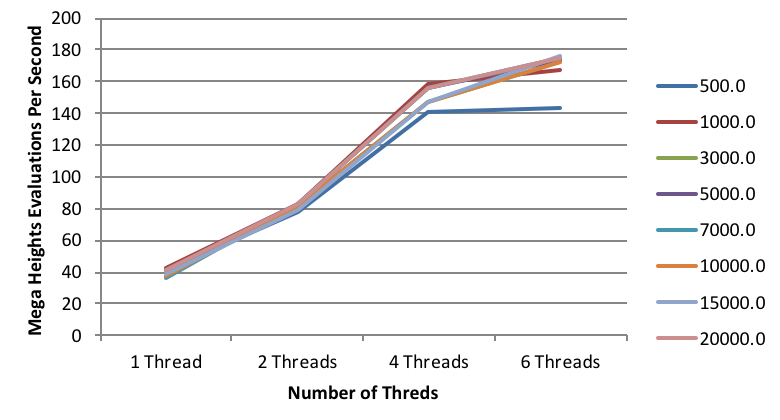
\includegraphics[width=18cm]{megasVthreads}
		\centering
	\end{figure}


\clearpage

\section{What patterns are you seeing in the speeds?}
	The coarse-grained parallelism for both static and dynamic scheduling increases from one to four threads, and then decreases after. The fine-grained parallelism decreases dramatically as the number of threads increases. In both pairs, the static scheduling is faster than the dynamic scheduling.
	
	
\section{Why do you think it is behaving this way?}
	I think the coarse-grained parallelism with static scheduling is faster than coarse-grained parallelism with dynamic scheduling, because this situation is better suited for static scheduling. In static scheduling, OpenMP assigns each thread a set of loop iterations to execute when it enters the parallel block. In dynamic scheduling, OpenMP assigns one iteration to each thread and when it finishes it gets assigned another. This results in dynamic scheduling having more overhead. Dynamic scheduling is better suited for a loop where each iteration may vary in execution time. Since this isn't in the case in this assignement, the dyanmic scheduling is adding unnecessary overhead. The overhead can be seen in the gap between the coarse+static and coarse+dynamic curves in the figure above.
	
	As for why the speed decreases after four threads, I'd assume that there isn't enough work to be done in the for-loops that the overhead of managing more than four threads doesn't pay off in terms of performance. I'd also assume that the coarse+dynamic curve decreases in speed due to additional threads adding to the overhead discussed above.

	I think that the speed in the fine-grained parallelism decreases dramatically with an increase in the number of threads because of the repetitive setup and destroy functionality taken on the thread pool. On each iteration the outer for-loop initiates the thread pool, and then destroys them at the end, and there isn't enough work done in the inner for-loop to make that overhead worthwhile.
	



\end{document}